% WSCG sample document 
%
% based on Gabriel Zachmann's sample
% http://zach.in.tu-clausthal.de/latex/
%
% modified Apr 2012 to match WSCG Word template
%
\documentclass[twoside,twocolumn,10pt]{article}
%\documentclass[twoside,twocolumn,draft]{article}

%  for debugging
%\tracingall%\tracingonline=0
%\tracingparagraphs
%\tracingpages


%%%%%%%%%%%%%%%%%%%%%%%%%%%%%%%%%%%%%%%%%%%%%%%%%%%%%%%%%%%%%%%%%%%%%%%%%%%%%
%                             Packages

\usepackage{wscg}           % includes a number of other packages (e.g., myalgorithm)
\RequirePackage{ifpdf}
\ifpdf
 \RequirePackage[pdftex]{graphicx}
 \RequirePackage[pdftex]{color}
\else
 \RequirePackage[dvips,draft]{graphicx}
 \RequirePackage[dvips]{color}
 \fi
\usepackage{subfig}
 
%\usepackage[german,english]{babel}     % default = english
%\usepackage{mypicture}      % loads graphicx.sty, color.sty, eepic.sty
%\usepackage{array}          % better tabular's & arrays, plus math tabular's
%\usepackage{tabularx}      % for selfadjusting p-columns
%\setlength{\extrarowheight}{1ex}   % additional space between rows
%\usepackage{booktabs}      % typographically much better
%\usepackage{mdwlist}        % for compacted lists, and more versatile lists
%\usepackage[intlimits]{amsmath} % more math stuff, see texdoc amsldoc
%\usepackage{mymath}         % own commands, loads amssymb & array.sty
%\usepackage{hyphenat}      % hyphenatable -, /, etc.
%\usepackage{theorem}
%\usepackage[sort&compress]{natbib}% better \cite commands, more flexible
%\usepackage[sort&compress,super]{natbib} % better \cite commands, more flexible
%\newcommand{\citenumfont}[1]{\textit{#1}}


\usepackage{nopageno}       % no page numbers at all; uncomment for final version
\usepackage{wrapfig}
\usepackage{moreverb}
\usepackage{algorithm2e}



%%%%%%%%%%%%%%%%%%%%%%%%%%%%%%%%%%%%%%%%%%%%%%%%%%%%%%%%%%%%%%%%%%%%%%%%%%%%%
%                                Title

\title{Estimating landmarks on 2D images of beetle mandibles}

\author{\hspace{-0.5cm}
\parbox{0.18\textwidth}{\centering
L\^e V\~anh L.\\[1mm]
ITDLU \\
 Dalat University \\
 Vietnam\\[1mm]
linhlv@dlu.edu.vn
}
\hspace{0.0\textwidth}
\parbox{0.2\textwidth}{\centering
Beurton-Aimar M.\\[1mm]
LaBRI- CNRS 5800\\
Bordeaux University \\
33400 Talence - F.\\[1mm]
beurton@labri.fr
}
\hspace{0.0\textwidth}
\parbox{0.2\textwidth}{\centering
Salmon J.-P.\\[1mm]
LaBRI- CNRS 5800\\
Bordeaux University \\
33400 Talence - F.\\[1mm]
jean-pierre.salmon@labri.fr
}
\hspace{0.0\textwidth}
\parbox{0.2\textwidth}{\centering
Marie A. \\[1mm]
IGEPP\\
INRA 1349\\
35653 Le Rheu - F.\\[1mm]
alexia.marie/nparisey
}
\hspace{0.0\textwidth}
\parbox{0.2\textwidth}{\centering
Parisey N.\\[1mm]
IGEPP\\
INRA 1349 \\
35653 Le Rheu - F.\\[1mm]
\hspace{-0.8cm}@rennes.inra.fr
}
}

%%%%%%%%%%%%%%%%%%%%%%%%%%%%%%%%%%%%%%%%%%%%%%%%%%%%%%%%%%%%%%%%%%%%%%%%%%%%%
%                          Hyperref


% no hyperlinks
\usepackage{url}
\usepackage{here}
\urlstyle{tt}

% Donald Arsenau's fix for missing kerning of "//" and ":/"
\makeatletter
\def\Uslash{\mathbin{\mathchar`\/}\@ifnextchar{/}{\kern-.15em}{}}
\g@addto@macro\UrlSpecials{\do \/ {\Uslash}}
\def\Ucolon{\mathbin{\mathchar`:}\@ifnextchar{/}{\kern-.1em}{}}
\g@addto@macro\UrlSpecials{\do : {\Ucolon}}
%%\Makeatother
 




%%%%%%%%%%%%%%%%%%%%%%%%%%%%%%%%%%%%%%%%%%%%%%%%%%%%%%%%%%%%%%%%%%%%%%%%%%%%%
%                              My Commands


%\DeclareMathOperator{\sgn}{sgn}

%\theorembodyfont{\upshape}
%\theoremstyle{break}
%\theoremheaderfont{\bfseries\normalsize}

%\newtheorem{lem}{Lemma}
%\newtheorem{defn}{Definition}



%%%%%%%%%%%%%%%%%%%%%%%%%%%%%%%%%%%%%%%%%%%%%%%%%%%%%%%%%%%%%%%%%%%%%%%%%%%%%
%                                Document


\begin{document}

\twocolumn[{\csname @twocolumnfalse\endcsname

\maketitle  % full width title


\begin{abstract}
    
Studying links between phenotype/genotype and agricultural practices is one of
the main topics in agronomy research. Phenotypes can be characterized
by informations like age, sex of animals/plants and more and more
often with the help of image analysis of their morphology. From now, getting good
quality of images for numerous individuals is easy but that leads to
design automatic procedures to replace manual exploration of such
amount of images. Several bottlenecks have been identified to analyze
automatically images. One of them is segmentation of selected area
and/or shapes, and another well-known one is setting automatically
morphometric landmarks. Landmarks are points on the object which can be used to identify or
to classify the objects.
\\
It exists a lot of methods to experiment landmarks setting, depending
on the image contents. This work has been initiated by using the
article of Palaniswamy et al. \textit{"Automatic identification
  of landmarks in digital
  images"}\cite{palaniswamy2010automatic}. They proposed a method
based on calculus of a probabilistic Hough transform coupling to a
template matching algorithm. They applied their method
to the Drosophilia wings. In our study, we have gotten a set of $291$ 
beetles . For each one $2$D images of $5$ different parts of their anatomy
have been taken: mandibles left and right, head, pronotum and
elytra. The first part of the project was to test how the
Palaniswamy's method could be used to analyze them. We have implemented  
all the required algorithms to compute positions of mandibles
landmarks and compared the obtained results to landmarks which have been manually set by biologists. We
will see that even positions automatically obtained are not fully precised, if we
used centroid size to characterize mandibles, the size computed from
automatic landmarks is closed to this one computed from the manual
ones. Future works will focus on definition of a
semi-landmarks procedure which would add some
features as the measure of the curve between two landmarks.

\end{abstract}

\subsection*{Keywords}
 Landmarks identification, probabilistic Hough transform, morphometry
 of beetle mandible.

\vspace*{1.0\baselineskip}
}]



%%%%%%%%%%%%%%%%%%%%%%%%%%%%%%%%%%%%%%%%%%%%%%%%%%%%%%%%%%%%%%%%%%%%%%%%%%%%%


\section{Introduction}

\copyrightspace
Morphology analysis is a way to characterize biological shape
variations. In the aim to study potential links between these
variations and agricultural ecosystems, a set of $291$ beetles has been collected. Informations as
sex, place where they were found and agricultural practices in
this field were set. To grow richer phenotype data, morphometric
operations could be done. To do that, a set of landmarks has been
defined. Morphometric landmarks are points that can be defined in all specimens and
located precisely \cite{web2010}. Landmarks are widely used in many biological
studying and analysis of geometric characteristics are currently included
into classification procedures.

~\\
\begin{figure}[h!]
\centering
\subfloat[Right mandible]
{\label{fig:example_111}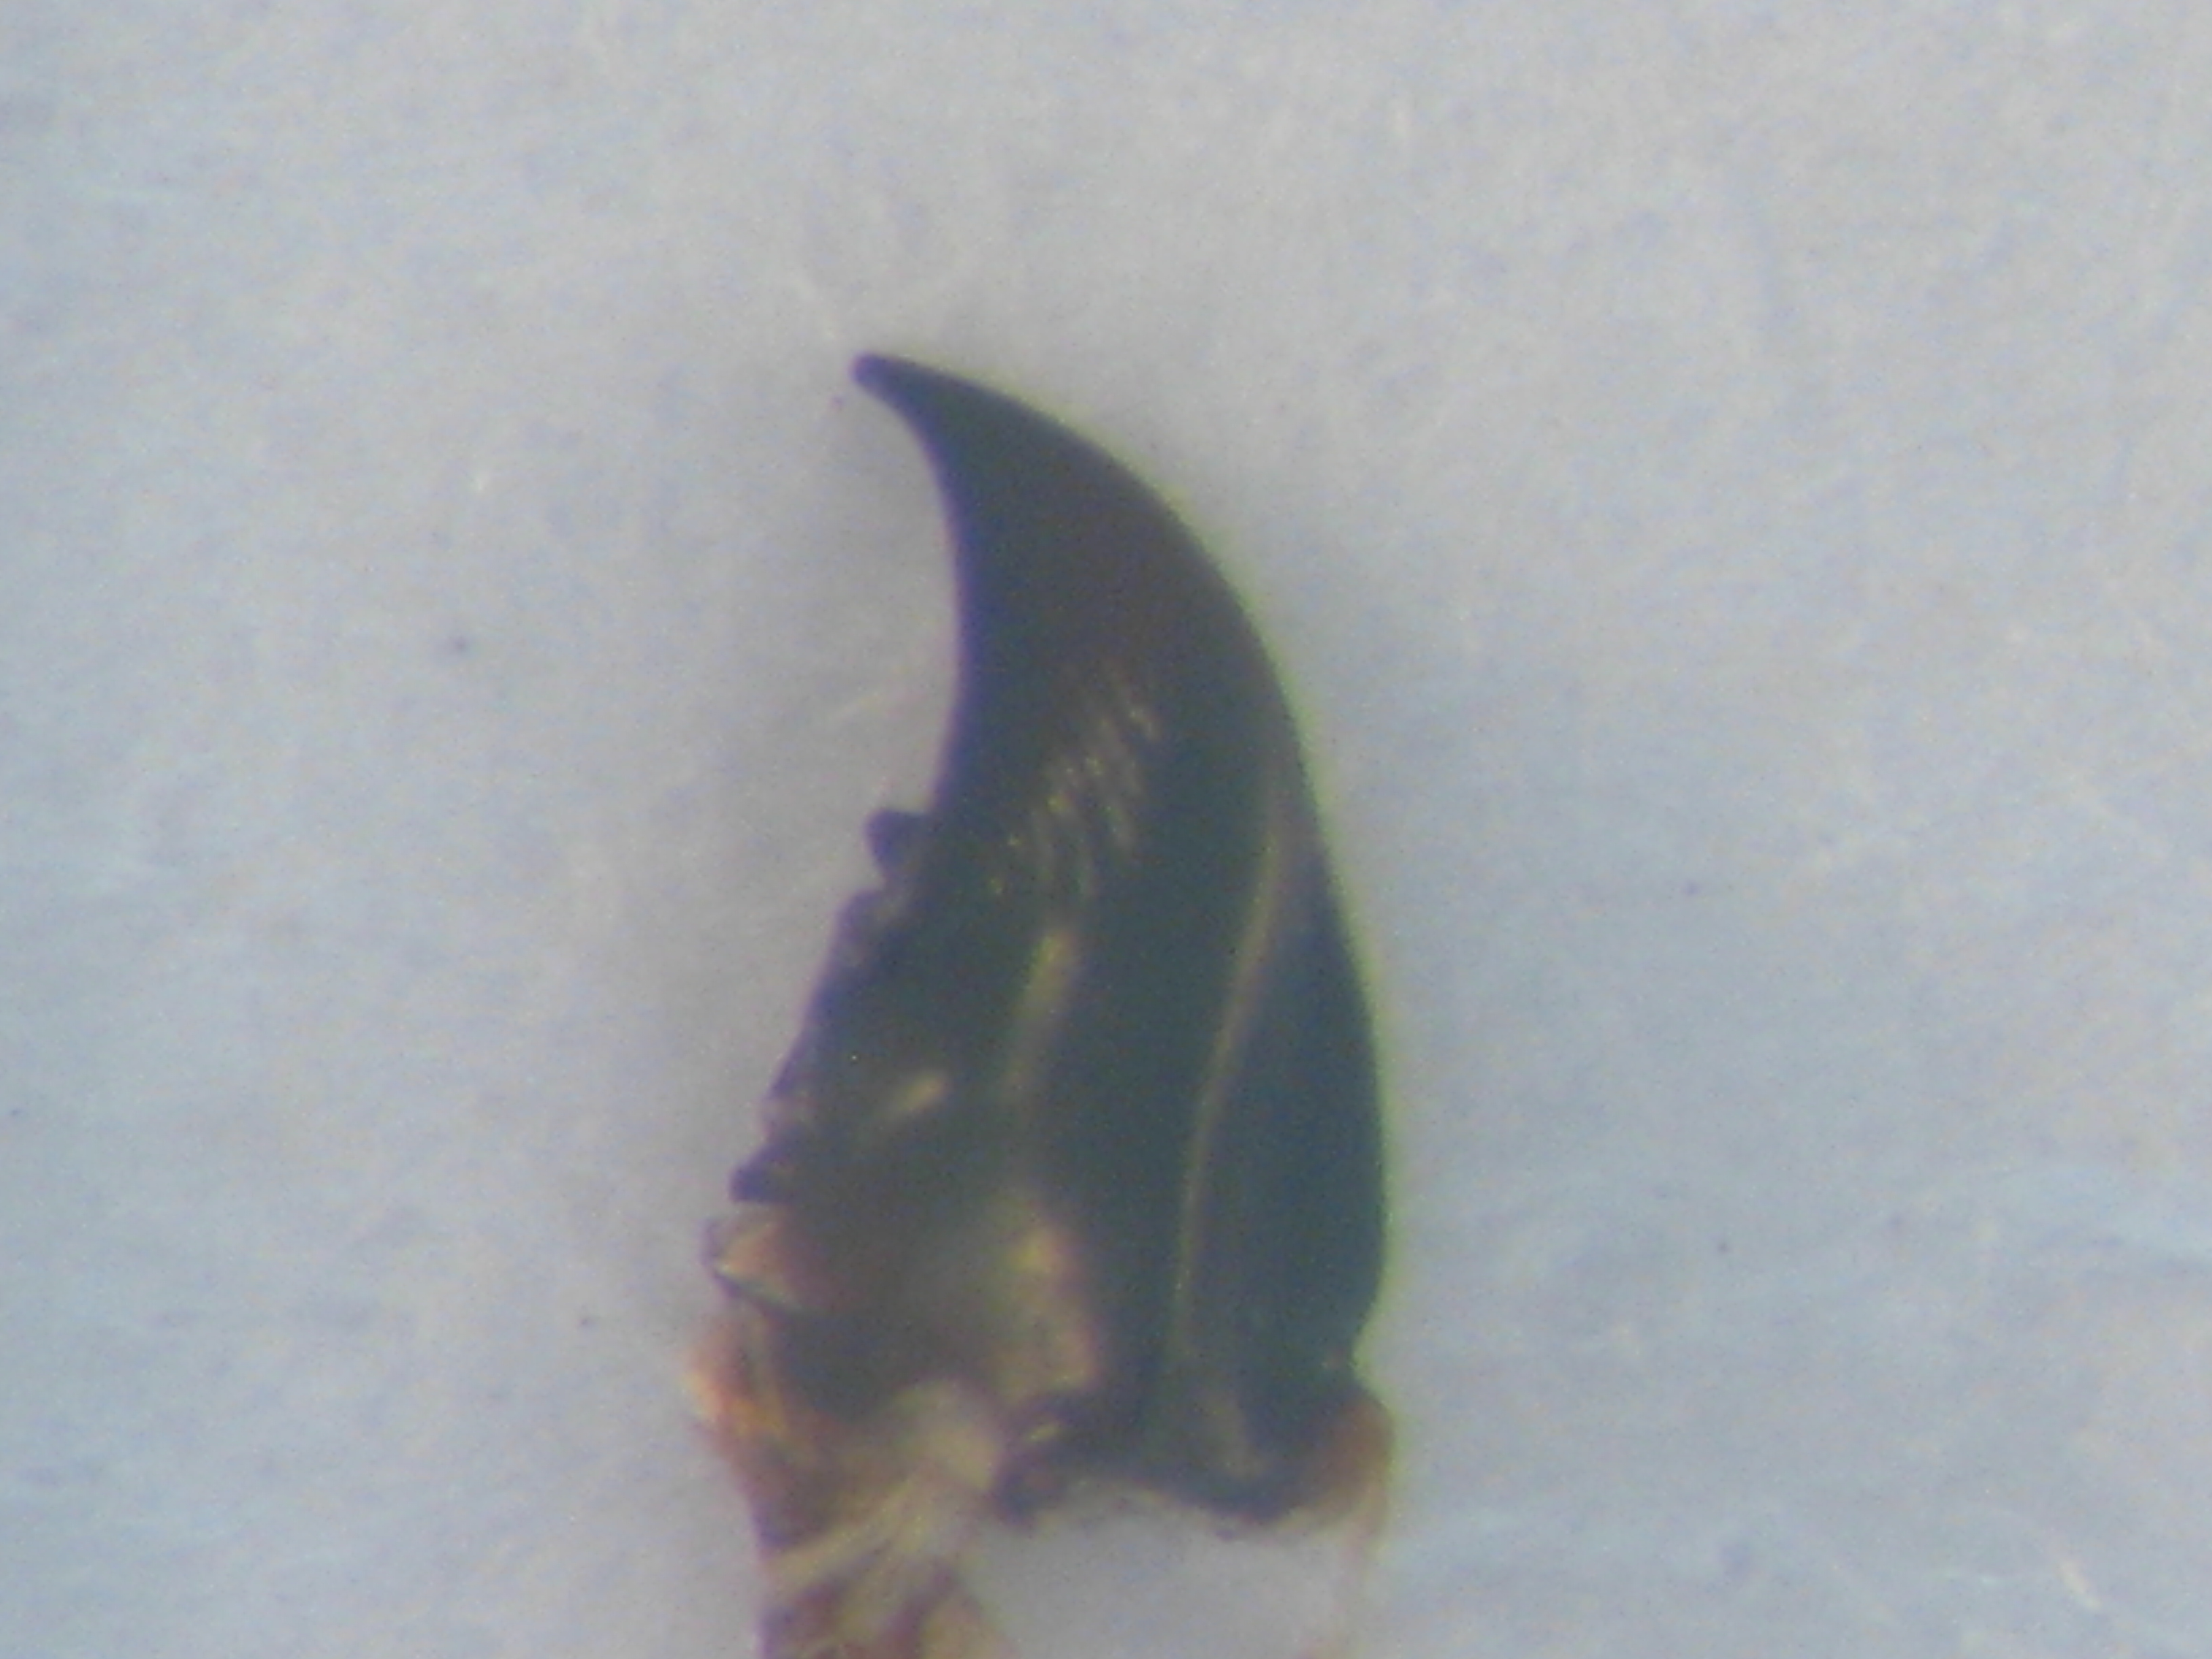
\includegraphics[width=0.22\textwidth]{./images/md32}}~~
\subfloat[Left mandible]
{\label{fig:example_112}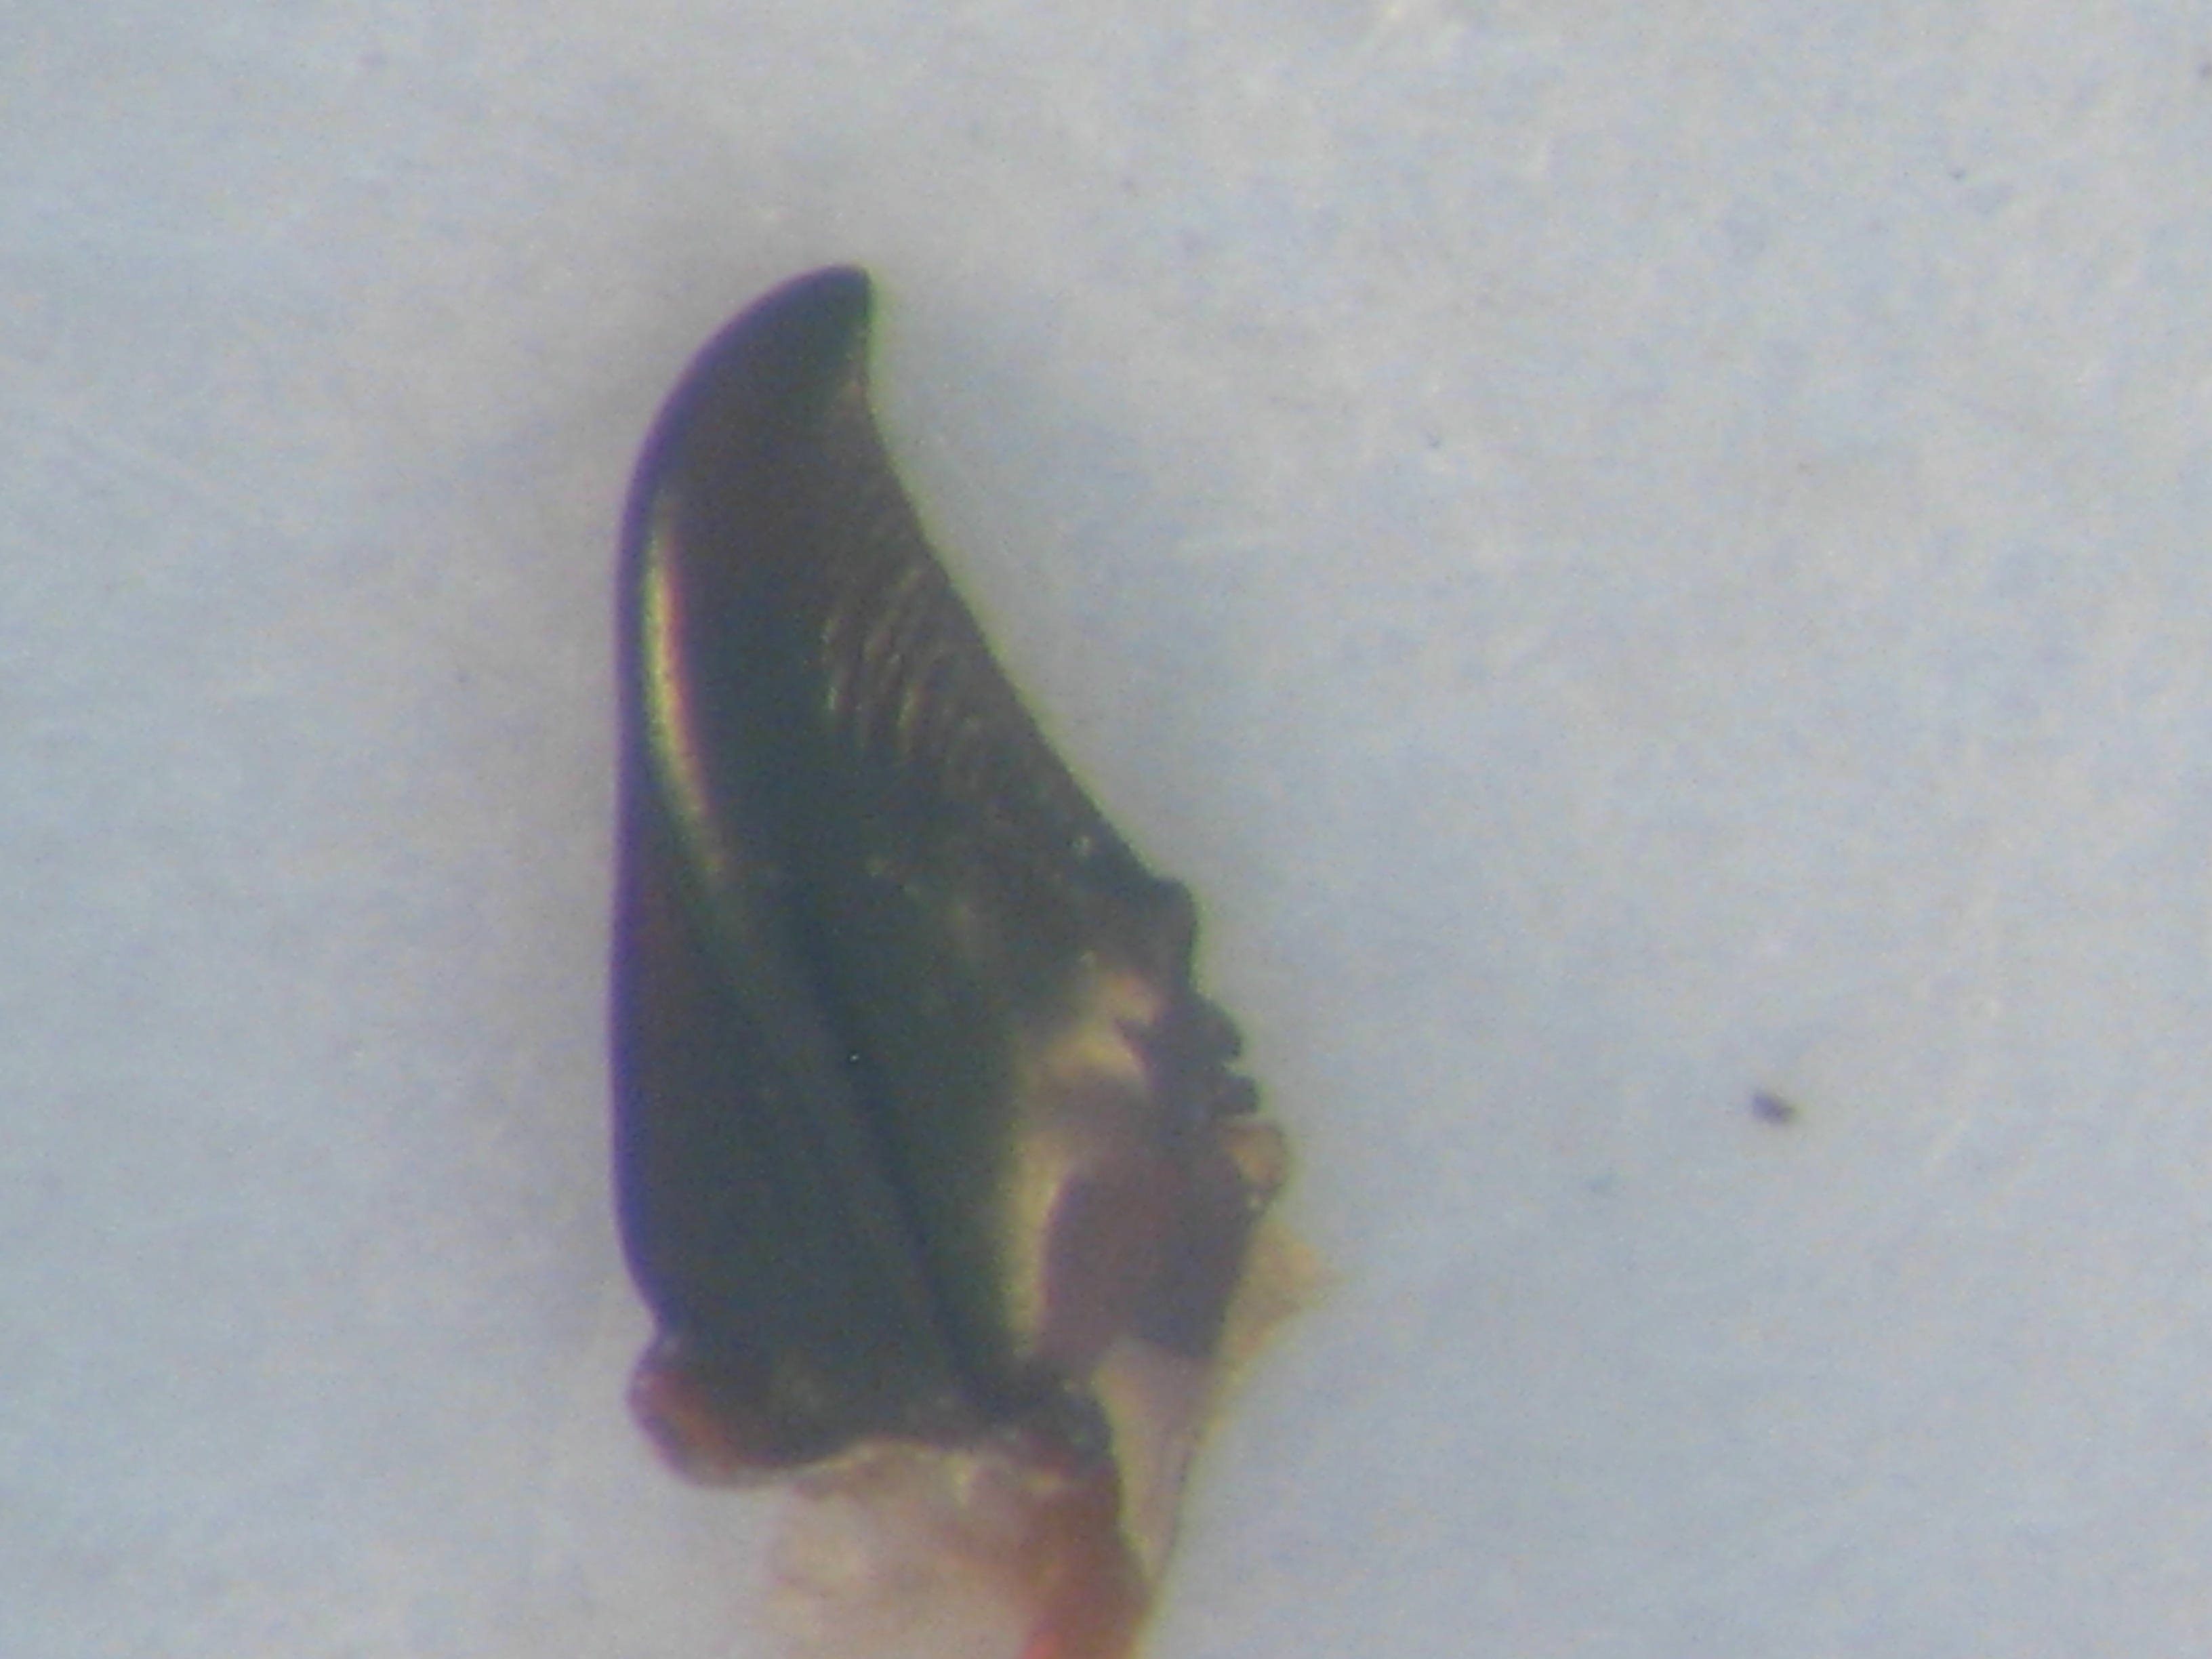
\includegraphics[width=0.22\textwidth]{./images/mg29}}
\caption{The mandibles of beetle}
\label{fig:figure_11}
\end{figure}
\\
In this paper, we focus on a method which addresses automatic identification of
landmarks in digital images. Palaniswamy et
al. \cite{palaniswamy2010automatic} have proposed a method to set landmarks
on images of Drosophila wings. We have investigated how this method can be
implemented to work on images of beetle mandibles (figure
\ref{fig:figure_11}). The method contains four stages: a features extraction of mandible
structure (segmentation stage), a recording of the features using pairwise
geometric histogram (PGH), an estimation of the landmarks positions using
Probabilistic Hough Transform (PHT) and finally a refinement of the estimated
landmarks by cross-correlation.

\section{Methods}
For each mandible image, a set of $18$ landmarks have been 
manually set by biologists corresponding to morphological points of
interest (see figure \ref{fig:segmentation}). It will constitute our ground truth. 
\begin{wrapfigure}{r}{4cm}
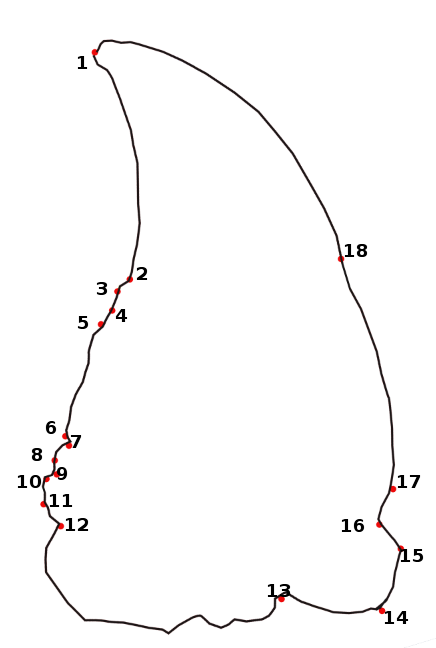
\includegraphics[width=4cm]{./images/rshape1}
\caption{\small{Manual landmarks of the right mandible}\label{fig:segmentation}}
\end{wrapfigure}
The automatic procedure to estimate these positions extracts
features by analyzing the image histogram firstly. The obtained
parameters are then used to approximate edges of the
mandible by line segments. These edges are presented to PGH
using geometric relationships between them. The shape correspondence
is determined by comparing the PGHs of model and scene data. A PHT 
is then used to identify hypothetical location of model landmarks on scene
image. Finally, the hypothetical landmarks are performed by template
matching. We now describe in details all these steps.

\paragraph{Segmentation step}
Usual way to obtain automatically threshold value for 
segmentation is to take a look to the image's histogram (figure
\ref{lm_hist}). 
\begin{wrapfigure}{r}{4.5cm}
\centering
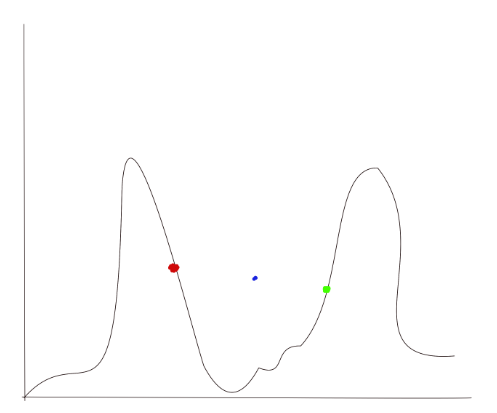
\includegraphics[width=4.5cm]{./images/hist}
\caption{\small{Image Histogram}}
\label{lm_hist1}
\end{wrapfigure}
In our case, per image we have only one object, the mandible,  into a
pretty uniform background, consequently the histogram exhibits only two
picks. In this case, the retained threshold value is the average 
value (blue point in fig.\ref{lm_hist1}) between two mean values (red and
green points in fig.\ref{lm_hist1}) of these two pick regions. The first region,
begins from the beginning to the median of histogram and the second region is the rest.\\
\\
The Canny algorithm \cite{canny1986computational} is one of the
relevant algorithms to detect segmentation edges. The result is a list
of points for each retrieved edge. To compute the PGH another kind of
geometric form, lines, is needed. Extraction of approximated lines
from the list of points can be achieved by using the
recursive algorithm \cite{thacker1995assessing}, which is a new improved version with the Lowe's method\cite{lowe1987three} as below:
{\small{\begin{description}
    \item[$\bullet$] Create a line connected by two edge endpoints
    \item[$\bullet$] For each point in the edge :
      \begin{description}
    		  \item[$\cdot$] Calculate the perpendicular distance from it to the line,
      	  \item[$\cdot$] Keep the point which have max distance, i.e. max point
 	 \end{description}
	  \item[$\bullet$] Divide edge at max point into two parts: the first part includes the points from the beginning endpoint to the max point and the last one is the points from the max point to  the endpoint.
      \item[$\bullet$] Repeat step 1 with two new parts of the edge.
  \end{description}
 } }
The algorithm stops when the edge cannot be broken more. Concretely,
we stop the algorithm when the maximum perpendicular distance of max
point is less than $3$ pixels, i.e. enough small to create an approximated line.

\paragraph{Comparison between model and scene}
In the previous stage, we convert the presented of edge from the list of points to the list of lines. It is useful to present the image in a compact and invariant. To determine the correspondence between the model and the scene image, we compute the similarity metric between two images. This value is indicated by comparing the PGH\cite{evans1993use} of the images.\\
The PGH is constructed from the geometric relationships of the lines (i.e relative angle and perpendicular distance). The relative angle is defined by angle between two lines; and the perpendicular distance uses the distance from two endpoints of the first line to the second line. With a line in image, we record the geometric relationships  between it and other lines in image when we consider it as reference line. It means that PGH of an image is combined from all PGHs of all lines in image.\\
The PGH is represented as a two dimension matrix with axis for relative angle and perpendicular distance. Each axis is divided into a number of rows (or columns) which determined by the expected accuracy of process. The steps to construct the PGH for an image as follows:
{\small{
\begin{description}
\item[$\bullet$] Create a matrix,
\item[$\bullet$] Choose a \textbf{reference line},
\item[$\bullet$] For each other lines in the shape,
	\begin{description}
		\item[$\cdot$] Calculating the perpendicular distance from two endpoints to the reference line,
		\item[$\cdot$] Computing the angle between the considered line and the reference line,
		\item[$\cdot$] Recording the perpendicular distance and angle into the matrix.
	\end{description}
\item[$\bullet$] Repeat step 2 (choose reference line) until all lines in the image are considered as reference lines.
\end{description}
}}
To be able to compare model and scene, a similarity metric
is needed. The Bhattacharya\cite{palaniswamy2010automatic} similarity
metric is used to compare the distribution (PGH) for the model and the
scene data. It computes the degree of match between them as a dot product correlation of the PGHs (equation \ref{eq:1}).
\begin{center}
\begin{equation} \label{eq:1}
d_{Bhatt} (H_{i}H_{j}) = \sum\limits_{\theta}^{\pi}\sum\limits_{d}^{d_{max}}\sqrt{H_{i}(\theta,d)H_{j}(\theta,d)}
\end{equation}
\end{center}
Where $H_{i}(\theta,d)$ is an entry at row $\theta$ (i.e. angle)  and
column $d$ (i.e. perpendicular distance) in the PGH of the image $i$.
 
\paragraph{Selection of matching points}
The Probabilistic Hough Transform (PHT) is then used to determined the presence and location of the
model in the scene image, as well as to determine the hypothesis of
the model landmarks in the scene
image\cite{ashbrook1995robust}. Applying PHT includes two steps:
first, we find the pair of scene lines that similar with a pair of
model lines (named training process); second, we estimate the model landmarks in the scene image.\\[0.2cm]
Training process includes the duration to construct the reference table for model image and process to find the similar pair of lines between model and scene image.\\
The reference table is created when we consider relative position between each pair of lines in model image and an arbitrary point(i.e reference point). It contains the relative information (angle and distance) from each line of pair to the reference point. The angle is angle between horizontal axis (begin from reference point) and perpendicular line from the reference point to the line. The distance is perpendicular distance from the reference point to the line. The steps to construct the reference table as follows:

{\small{
	\begin{description}
		\item[$\bullet$] Create the table to record relative information (3 columns\footnote{The first column contains pair of lines, two last columns contain the relation position of each line (in pair of lines)with reference point}),
		\item[$\bullet$] Choose the reference point in model,
		\item[$\bullet$] For each pair of model lines, calculate the distance and angle from each line to the point and save into the table.
	\end{description}
}}
After obtaining the reference table of model image, we consider the presence of the model in the scene image by finding the similar pair of lines between them. And a probabilistic statistical is applied to finish this work. With the ``vote'' for each similar pair between model and scene, we will obtain the pair of lines have the largest ``vote'' value, and there is the pair of scene line similar with pair of model. The steps to find the similar pair of lines between model and scene image as follows:
{\small{
\begin{description}
	\item[$\bullet$] Create an accumulator (a two dimension matrix (angle and perpendicular distance)),
	\item[$\bullet$] For each pair of scene lines, find the pair of model lines within correspondence in position, orientation and scale. Select the respective value (relative information) in reference table,
	\item[$\bullet$] Increase the value in accumulator at respective position and keep the cell that have the maximum value.
\end{description}
}}
The pair of scene lines having the best value is chosen. The presence of the reference point (of model) in the scene\cite{ashbrook1995robust} image is indicate by the respective information from the reference table. The estimated landmarks in the scene obtained by calculating the relatedness between
the model's reference point and the model's landmarks are
recorded. Besides, we also record the difference angle between model
image and the scene image. Fig. \ref{fig:figure_12} shows an example
of result, the red points are estimated landmarks on the scene mandible
(right one) from a model mandible (left one) landmarks. 
\begin{figure}[h!]
\centering
\subfloat[The model image]
{\label{fig:example_121}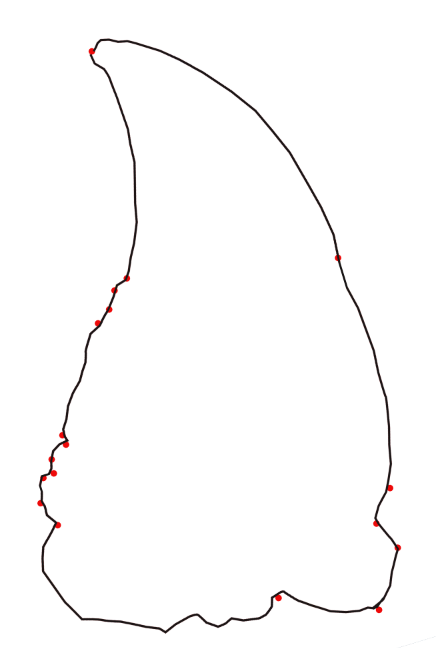
\includegraphics[width=0.18\textwidth]{./images/rshape}}~~
\subfloat[The scene image]
{\label{fig:example_122}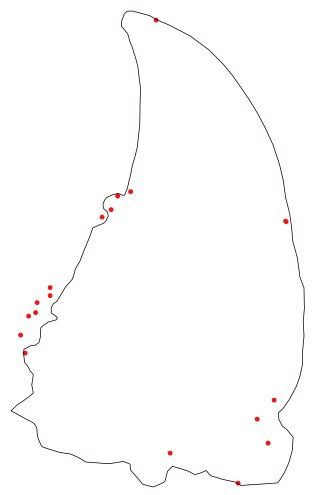
\includegraphics[width=0.18\textwidth]{./images/training}}
\caption{The estimated landmarks by PHT}
\label{fig:figure_12}
\end{figure}
\paragraph{Template matching}
The template matching is process to verify the landmarks estimation
provided in the PHG stage. Cross-correlation method\cite{knapp1976generalized} is hired for this work. By sliding the template on image by each pixel, cross-correlation will detect the best similarity between model and scene image. To save time during work, we should rotate the scene image to match with the model image (follows difference angle from PGH stage) and we just consider in a square around the landmarks (instead over image) when applying the cross-correlation. The progress of template matching as follows:
{\small{
\begin{description}
\item[$\bullet$] Rotate the scene image (the angle has indicated by PHT),
\item[$\bullet$] Create a bounding box around a model manual landmark (in model image),
\item[$\bullet$] Create a bounding box around a estimated landmark (in scene image) (the size of this box should larger than the size of box in model image),
\item[$\bullet$] Apply cross-correlation between the two bounding boxes.
\end{description}
}}
The template matching finishes when all estimated landmarks are
refined. Fig \ref{lm_hist} shows a complete result on one scene
mandible with the segmentation (red lines), manual landmarks (yellow
points) and estimated landmarks (green points).
\begin{figure}[h!]
\centering
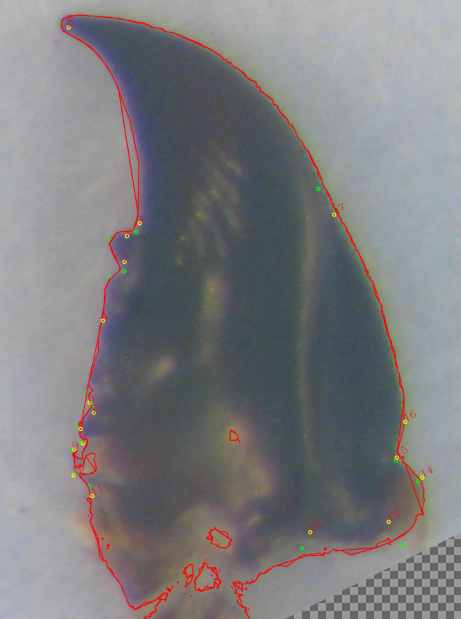
\includegraphics[width=7cm]{./images/Screenshot3.png}
\caption{\small{Automated landmarks in scene image after refining}}
\label{lm_hist}
\end{figure}
\section{Experiments and results}
All the algorithms have been implemented in a framework MaeLab in C++
language\footnote{MaeLab is a free software, it can be directly obtained
 by request to the authors.}. The set of beetles images have
been analyzed, right mandibles have been first studied. After
verification of the image correctness, it remains $288$ usable 
images. From the $3$ images removed, $2$ do not contain mandible and
in the last one, the mandible is broken in $2$ parts. All valid 
images have been segmented and the $18$ landmarks have been set
for each. Biologists have chosen to use in a first attempt the centroid
size to measure the mandible. This size is obtained by determination of the
centroid of the mandible and by sum of all square distances 
between each landmark and the centroid (see \cite{web2010} for
details).
\begin{figure}[h!]
\centering
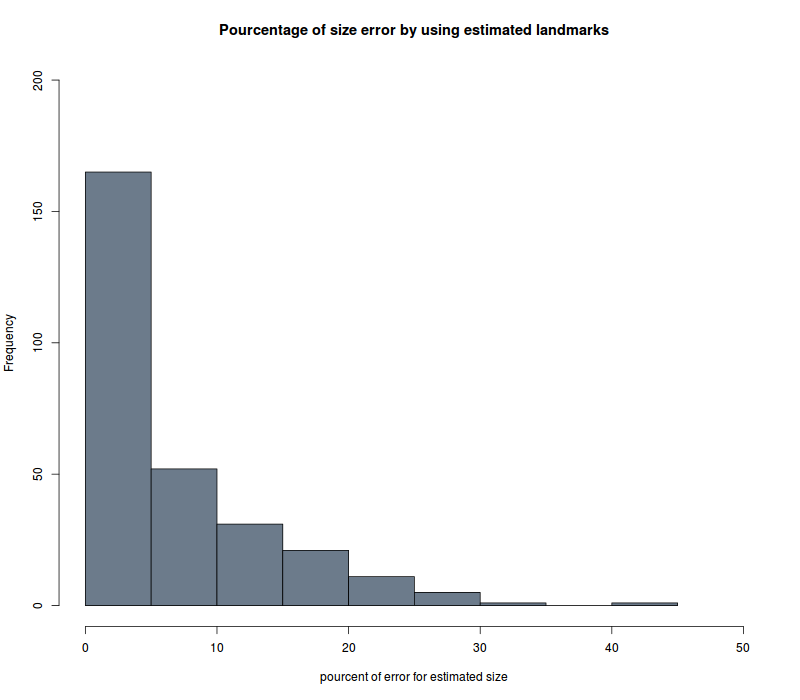
\includegraphics[width=7cm]{./images/frequency.png}
\caption{\small{Percentage of error in computing centroid size from estimated
landmarks}}
\label{percentage}
\end{figure}

In that way, we have compared the size computed from manual landmarks and this one from estimated
landmarks. The percentage of errors has been evaluated as below: 
{\small{
$$
PercentOfErr = \frac{100 \star |(Original Size - Estimated Size)|}{ Original Size}
$$
}}
We can observe in fig. \ref{percentage} that for more than $150$ images, the error
is less than $5\% $. Only $2$ mandibles could be considered as wrongly
measured with the estimated landmarks and exhibit more than  $30\% $
of errors. Finally $90\% $ of images have less than $10\% $ of error in
their size computing and for which we can consider estimated landmarks
as good enough to replace manual landmarks.

\paragraph{Perspectives and future works}
Of course, centroid size is not the only feature we want to
consider. It is also possible to compare image per image the exact
position of manual and estimated landmarks, for example if we want to
work with semi-landmarks by adding of curve measure between $2$
landmarks.

In our case, the landmark couples $1$ and $2$ or $1$ and $17$ (figure
\ref{fig:segmentation}) are good candidates to play this role. Figure
\ref{lm_hist} shows for one mandible the results which have been obtained
for each landmark. What one can note is that for some of them, an
offset appears. For example 
\section{Conclusion}
Morphometric analysis is a powerful tool in biology in order to
characterize species. Unfortunately, setting landmarks to run such
analysis is time consuming and difficult to replicate through
different experiments. In this project we have begun to design set of
procedures to segment $288$ beetle mandibles and to identify automatically
landmarks which have been described by biologists. Each mandible is
segmented by computing a approximated lines set. Using the
Probabilistic Hough Transform method, these lines are
used to align all mandibles scenes with one mandible model. The
first results shows that in order to compute the mandible centroid
size, the estimated landmarks are accurately enough. A framework in
C++ language has been developed to facilitate the using
to biologists. From now, a next stage of this studying is to add features as measure of curves,
in that way the landmark positions have to be set more precisely. To
solve this problem, algorithms based on design of shape skeleton will
be tried.


\bibliographystyle{plain}
\bibliography{./includes/references}
\end{document}
%-------------------------------------------------------------------------

\begin{thebibliography}{99}


\bibliography{./includes/references}
%\bibliographystyle{plain}
\end{thebibliography}

{\bfseries
Last page should be fully used by text, figures etc. Do not leave empty space, please. 

Do not lock the PDF -- additional text and info will be inserted, i.e. ISSN/ISBN etc. 
}


\end{document}

